\documentclass[]{article}
\usepackage{graphicx}
\usepackage[svgnames]{xcolor} 
\usepackage{fancyhdr}
\usepackage{tocloft}
\usepackage[export]{adjustbox}
\usepackage{graphicx}
\usepackage[hidelinks]{hyperref}
\usepackage{enumitem}
\usepackage{wrapfig}
\usepackage[many]{tcolorbox}
\usepackage{listings }
%\usepackage[a4paper, total={6in, 8in} , top = 2cm,bottom = 4cm]{geometry}
\usepackage[a4paper, total={6in, 8in}]{geometry}
\usepackage{afterpage}
\usepackage{amssymb}
\usepackage{pdflscape}
\usepackage{textcomp}
\usepackage{xecolor}
\usepackage{rotating}
\usepackage[Kashida]{xepersian}
\usepackage[T1]{fontenc}
\usepackage{tikz}
\usepackage[utf8]{inputenc}
\usepackage{PTSerif} 
\usepackage{seqsplit}
\usepackage{changepage}


\usepackage{listings}
\usepackage{xcolor}
\usepackage{sectsty}

\setcounter{secnumdepth}{0}
 
\definecolor{codegreen}{rgb}{0,0.6,0}
\definecolor{codegray}{rgb}{0.5,0.5,0.5}
\definecolor{codepurple}{rgb}{0.58,0,0.82}
\definecolor{backcolour}{rgb}{0.95,0.95,0.92}
\definecolor{blanchedalmond}{rgb}{1.0, 0.92, 0.8}
\definecolor{brilliantlavender}{rgb}{0.96, 0.73, 1.0}
\definecolor{CustomColor}{HTML}{cc0000}
 
\NewDocumentCommand{\codeword}{v}{
\texttt{\textcolor{blue}{#1}}
}
\lstset{language=java,keywordstyle={\bfseries \color{blue}}}

\lstdefinestyle{mystyle}{
    backgroundcolor=\color{backcolour},   
    commentstyle=\color{codegreen},
    keywordstyle=\color{magenta},
    numberstyle=\tiny\color{codegray},
    stringstyle=\color{codepurple},
    basicstyle=\ttfamily\normalsize,
    breakatwhitespace=false,         
    breaklines=true,                 
    captionpos=b,                    
    keepspaces=true,                 
    numbers=left,                    
    numbersep=5pt,                  
    showspaces=false,                
    showstringspaces=false,
    showtabs=false,                  
    tabsize=2
}

\lstset{style=mystyle}

 \settextfont[BoldFont={XB Zar bold.ttf}]{XB Zar.ttf}


\setlatintextfont[Scale=1.0,
 BoldFont={LiberationSerif-Bold.ttf}, 
 ItalicFont={LiberationSerif-Italic.ttf}]{LiberationSerif-Regular.ttf}





\newcommand{\inputsample}[1]{
    ~\\
    \textbf{ورودی نمونه}
    ~\\
    \begin{tcolorbox}[breakable,boxrule=0pt]
        \begin{latin}
            \large{
                #1
            }
        \end{latin}
    \end{tcolorbox}
}

\newcommand{\outputsample}[1]{
    ~\\
    \textbf{خروجی نمونه}

    \begin{tcolorbox}[breakable,boxrule=0pt]
        \begin{latin}
            \large{
                #1
            }
        \end{latin}
    \end{tcolorbox}
}

\newtcolorbox{mybox}[2][]{colback=red!5!white,
colframe=red!75!black,fonttitle=\bfseries,
colbacktitle=red!85!black,enhanced,
attach boxed title to top center={yshift=-2mm},
title=#2,#1}

\newenvironment{changemargin}[2]{%
\begin{list}{}{%
\setlength{\topsep}{0pt}%
\setlength{\leftmargin}{#1}%
\setlength{\rightmargin}{#2}%
\setlength{\listparindent}{\parindent}%
\setlength{\itemindent}{\parindent}%
\setlength{\parsep}{\parskip}%
}%
\item[]}{\end{list}}


\definecolor{foldercolor}{RGB}{124,166,198}
\definecolor{sectionColor}{HTML}{ff5e0e}
\definecolor{subsectionColor}{HTML}{008575}

\definecolor{listColor}{HTML}{00d3b9}

\definecolor{umlrelcolor}{HTML}{3c78d8}

\definecolor{subsubsectionColor}{HTML}{3c78d8}

\defpersianfont\authorFont[Scale=0.9]{XB Zar bold.ttf}

\defpersianfont\titr[Scale=1.5]{Lalezar-Regular.ttf}

\defpersianfont\fehrest[Scale=1.2]{Lalezar-Regular.ttf}

\defpersianfont\fehrestTitle[Scale=3.0]{Lalezar-Regular.ttf}

\defpersianfont\fehrestContent[Scale=1.2]{XB Zar bold.ttf}


\sectionfont{\color{sectionColor}}  % sets colour of sections
\subsectionfont{\color{subsectionColor}}  % sets colour of sections
\subsubsectionfont{\color{subsubsectionColor}}


\renewcommand{\labelitemii}{$\circ$}


\renewcommand{\baselinestretch}{1.1}


\renewcommand{\contentsname}{فهرست}

\renewcommand{\cfttoctitlefont}{\fehrestTitle}


\renewcommand\cftsecfont{\color{sectionColor}\fehrestContent\selectfont}
\renewcommand\cftsubsecfont{\color{subsectionColor}\fehrestContent\selectfont}
\renewcommand\cftsubsubsecfont{\color{subsubsectionColor}\fehrestContent\selectfont}
\renewcommand{\cftsecleader}{\cftdotfill{\cftdotsep}}
%\renewcommand{\cftsecpagefont}{\color{sectionColor}}

\setlength{\parskip}{1.2pt}

\begin{document}


%%% title pages
\begin{titlepage}
\begin{center}

\textbf{ \Huge{به نام خدا} }
        
\vspace{0.2cm}


\includegraphics[width=0.4\textwidth]{sharif1.png}\\
\vspace{0.2cm}
\textbf{ \Huge{\emph درس برنامه‌سازی پیشرفته} }\\
\vspace{0.25cm}
\textbf{ \Large{معماری \lr{P2P}} }
\vspace{0.2cm}
       
 
      \large \textbf{دانشکده مهندسی کامپیوتر}\\\vspace{0.1cm}
    \large   دانشگاه صنعتی شریف\\\vspace{0.2cm}
       \large   ﻧﯿﻢ سال دوم 99-98 \\\vspace{0.10cm}
      \noindent\rule[1ex]{\linewidth}{1pt}
اساتید:\\
    \textbf{{مهدی مصطفی‌زاده، ایمان عیسی‌زاده، امیر ملک‌زاده، علی چکاه}}



        \vspace{0.10cm}
نگارش و تهیه محتوا:\\
    \textbf{{صابر ظفرپور}}
    
       \vspace{0.10cm}
       تنظیم داک:\\
    \textbf{{امیرمهدی نامجو و صابر ظفرپور}}

    
        \vspace{0.05cm}
    

\end{center}
\end{titlepage}
%%% title pages


%%% header of pages
\newpage
\pagestyle{fancy}
\fancyhf{}
\fancyfoot{}
\cfoot{\thepage}
\lhead{Peer-to-Peer}
\rhead{
\includegraphics[width=0.1\textwidth]{sharif.png}\\
دانشکده مهندسی کامپیوتر
}
\chead{پروژه برنامه‌سازی پیشرفته}
%%% header of pages
\renewcommand{\headrulewidth}{2pt}

\KashidaOff



\tableofcontents

\newpage

 \Large \textbf{\\\\
}

\section*{{\titr اینو دیگه کجای دلمون باس جا بدیم؟}}
\addcontentsline{toc}{section}{{\fehrestContent اینو دیگه کجای دلمون باس جا بدیم؟}}


یکی بود ولی هنوز اینترنت نبود، اواخر دهه هفتم قرن 20ام میلادی پروژه‌ای مشترک بین تعدادی از دانشگاه‌های آمریکا و به واسطه پشتیبانی \lr{DoD} (وزارت دفاع آمریکا) آغاز به کار کرد که 4 راس در نقاط مختلف آمریکا را به یکدیگر وصل کرد. بعدها این شبکه گسترش یافت و با نام اینترنت به صورت تجاری و برای عموم مردم قابل استفاده شد. در اوایل این دوران معماری که مورد استفاده قرار می‌گرفت چیزی نبود جز یک معماری \lr{P2P} ، اما با گذر زمان به علل مختلف (امنیتی ، تجاری ، فنی و …) معماری مورد استفاده توسط اینترنت طی یک دگرگونی تبدیل به چیزی شد که ما الان با آن آشنایی داریم .

\begin{center}
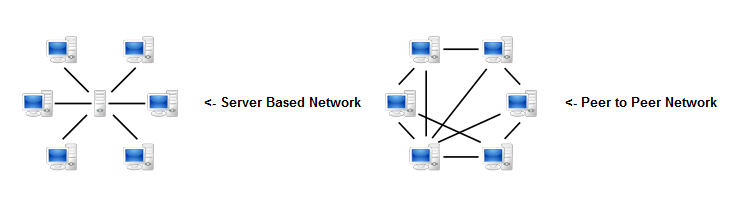
\includegraphics[width=1\textwidth]{images/i0.png}
\end{center}

معماری بر مبنای مدل کلاینت سرور مدلی از معماری شبکه است که در حال حاضر به صورت کاملا وسیعی مورد استفاده قرار گرفته است. در این مدل تعدادی سرور وجود دارد که بقیه کاربران فقط حق ارتباط مستقیم با همین سرورها را دارند ، به طور مثال فرض کنید شما (\lr{Alice}) در این مدل قصد دارید برای دوست خود(\lr{Bob}) یک فایل موزیک را ارسال کنید، احتمالا تمام راه‌های انتقال فایلی که در ذهن دارید از طریق همین نوع معماری است (تقریبا تمامی نرم افزارهای فضای ابری و یا پیام‌رسان‌ها) ، اما سوالی که در ذهن ایجاد می‌شود اینست که آیا واقعا این مدل معماری شبکه در تمامی حالات منطقی است؟؟؟ چرا در چنین شبکه‌ای (اینترنت)که تمامی راس‌های عضو آن در یک گراف همبند قرار دارند، این راس‌ها نباید قادر به ارتباط مستقیم و بدون حضور شخص سوم با یکدیگر باشند؟( اگر این مسئله باعث دغدغه ذهنی شما نشده، خواندن ادامه داک احتمالا برای شما بی ثمر خواهد بود)

\begin{center}
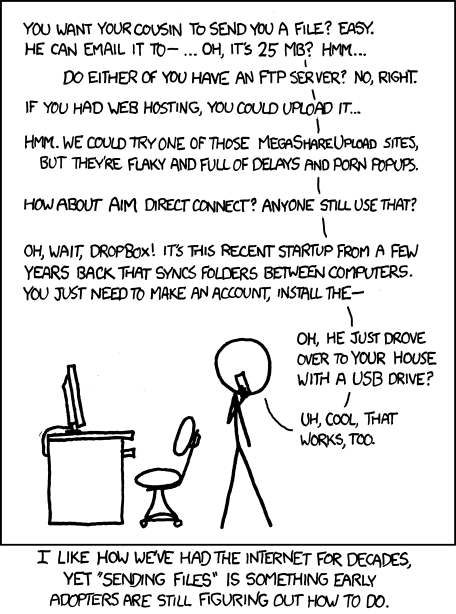
\includegraphics[width=0.8\textwidth]{images/file_transfer.png}
\end{center}


\section*{{\titr بازگشت به ریشه‌ها}}
\addcontentsline{toc}{section}{{\fehrestContent بازگشت به ریشه‌ها}}


در طی تمامی این سال‌ها ، توسعه دهندگان متن باز  \lr{(open-source developers)} بر روی ایده‌ها و پیاده‌سازی‌های خلاقانه p2p کار کرده‌اند. احتمالا نام بعضی از این ایده ها و ابزارها برایتان آشنا باشد (بیت کوین (واحد پول بدون بانک مرکزی)، بیت تورنت (اشتراک گذاری فایل در اینترنت)، \lr{Usenet} , \lr{Napster}  \lr{Darknet} ,\lr{Skype}, \lr{Gnutella}).


\begin{wrapfigure}{l}{0.5\textwidth}\centering
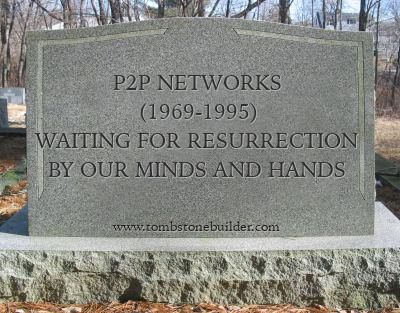
\includegraphics[width=0.5\textwidth]{images/i1.png}
\end{wrapfigure}

اگر هم این سنگ قبر برایتان سوالی ایجاد کرده و به دنبال قاتل این موجود شریف و اصیل هستید، شما را به این موجود (\lr{NAT}) ارجاع میدهم که باعث بسیار سخت شدن پیاده سازی این معماری در سطح اینترنت شده است. البته تا سال‌های 2005 نیز همچنان بیشتر ترافیک اینترنت توسط اپلیکیشن های با معماری \lr{P2P} مصرف میشد.
 
 
\section*{{\titr یکمی هم حرف فنی بزن دیگه!!}}
\addcontentsline{toc}{section}{{\fehrestContent یکمی هم حرف فنی بزن دیگه!!}}

در این معماری هیچ گونه تفاوتی بین راس‌ها وجود ندارد، یعنی هر راس هم می‌تواند سرور باشد و هم کلاینت ، یعنی می‌تواند همزمان که یک فایل را برای فرد دیگر میفرستد ، فایل مورد نیاز خود را از فرد دیگری در شبکه دریافت کند.

همانطور که احتمالا می‌دانید به هر موجود در شبکه یک شماره منحصر به فرد به نام IP داده می‌شود، اما این IP کافی نیست ، یک عدد دیگر نیز تعیین کننده است، این عدد port است،که از 0 تا 65535 بازه آن است، این عدد تعیین کننده این است که اگر بسته‌ای به IP شما ارسال شد باید برای کدام برنامه سیستم عامل ارسال شود (به طور مثال اگر شما همزمان در حال استفاده از دو مرورگر باشید، باید سیستم عامل بداند که هر بسته مربوط به کدام مرورگر است)، پس اگر شما بر روی یک پورت رندوم در حال شنیدن باشید و IP و آن پورت را به فرد دیگری بدهید‌، شما و آن فرد میتوانید به صورت مستقیم به هم وصل شوید و در صورت استفاده از پروتکل (مانند زبان مورد استفاده انسان‌ها) یکسان می‌توانید با هم ارتباط برقرار کنید.
البته ذکر این نکته ضروری است که این مسئله به علت وجود NAT نزدیک به 25 سال است که تبدیل به یک چالش شده است، البته تعدادی روش برای دور زدن این موجود \lr{(NAT Traversal)} به وجود آمده است که به وسیله آن هنوز می‌توانیم به ادامه این معماری امید داشته باشیم.
   تقسیم می‌شود.


\newpage
\section*{{\titr خب این Peer-to-Peer اصلا چه مزایایی داره؟؟}}
\addcontentsline{toc}{section}{{\fehrestContent خب این Peer-to-Peer اصلا چه مزایایی داره؟؟}}


هزینه راه اندازی سرور‌ها برای اکثریت سرویس‌ها یک بار اضافه و از نظر مالی بسیار سنگین است ، به طور مثال فرض کنید شما یک پیام‌رسان بومی تولید کرده‌اید و این پیام‌رسان قابلیت تماس تصویری دارد و همچنین فرض کنید در حال حاضر که همه در خانه‌های خود هستند (در زمان نگارش این داک کرونا شکست نخورده بود:) بیش از 50000 کاربر از قابلیت تماس تصویری شما استفاده کنند و با یکدیگر تماس برقرار کنند، اگر فرض کنیم ثانیه‌ای 300kb توسط هر راس اطلاعات به سرور برای فرستادن به راس دیگر فرستاده شود‌، آنگاه شما باید قادر به تامین گذردهی حداقل 15Tb در ثانیه برای سرور خود باشید که حتی بدون حساب کردن قدرت پردازشی تلف شده یک هزینه کاملا بی دلیل است، در صورت استفاده از یک معماری \lr{P2P} آنگاه دیگر نیاز به چنین سرور با چنین منابع بالایی نبود. نکته دیگر موضوع امنیت است که در این نوع معماری با توجه اینکه می‌توان رمز گذاری‌های متنوعی استفاده کرد، دغدغه امنیت ارتباط کاربران برطرف می‌شود. 
هرگز مزیت privacy موجود برای هر راس در این نوع شبکه را از یاد نبرید، این مزیت در کنار غیر قابل \textcolor{red}{سانسور} بودن‌، دو مزیت بسیار بسیار مهم این نوع معماری هستند.



\section*{{\titr  چطور یک Peer-to-Peer دولوپر شم؟}}
\addcontentsline{toc}{section}{{\fehrestContent چطور یک Peer-to-Peer دولوپر شم؟}}

کاملا واضح است که با توجه به شرایط فعلی (وجود NAT در اکثر شبکه‌ها)، شما نمی‌توانید همانند معماری سرور و کلاینت با چند خط کد ساده یک ساختار شبکه \lr{P2P} پیاده کنید. اما با مطالعه کد‌های موجود در مخازن گیت هاب به ایده‌های بسیار جذابی بر می‌خورید، پس یکی از منابع اصلی یادگیری \lr{P2P} کدهای موجود در گیت هاب است (میتوانید با جستجوی tag هایی نظیر \lr{P2P} به این \href{https://github.com/search?l=Java&q=p2p-network&type=Repositories}{\textcolor{blue}{\underline{مخازن}}}
 دسترسی داشته باشید) 


گوگل چندین سال است که در حال توسعه تکنولوژی به نام \href{https://webrtc.org/}{\textcolor{blue}{\underline{\lr{WebRTC}}}} است که در حال حاضر توسط اکثر دولوپر‌های این حوزه درحال استفاده است. \href{https://webtorrent.io/}{\textcolor{blue}{\underline{\lr{WebTorrent}}}} نیز بر روی ترکیب این تکنولوژی و تورنت ساخته شده است. در حال حاضر بهترین زبان برای پیاده سازی و استفاده از معماری \lr{P2P} زبان javascript (که هیچ ربطی به جاوا نداره) است.
البته توصیه می‌شود قبل از تلاش برای شروع کد زدن و پیاده سازی این معماری در ابتدا با مطالعه مفاهیم {\lr{NAT Traversal} و پروتکل‌های رایج مورد استفاده نظیر STUN ,TURN, ICE آشنایی حداقلی را با این موضوع به دست بیاورید.


\section*{{\titr پس پروژه چی شد این وسط؟؟}}
\addcontentsline{toc}{section}{{\fehrestContent معماری Peer-To-Peer}}

در فاز سه، قسمتی امتیازی وجود دارد که شما باید برای قسمت فروش فایل، از این معماری به صورت محدود (فقط برای انتقال فایل) استفاده کنید ، به این صورت که خریدار فایل خود را از سرور دریافت نکند بلکه آن را به صورت مستقیم از فروشنده دریافت کند.
\begin{enumerate}
\item
برای بررسی کردن و نمره دادن به این بخش، به پیاده سازی پروتکل و برقراری ارتباط نمراتی تعلق می گیرد (پس با کمی وقت گذاشتن می‌تونید از این قسمت امتیازی نمره مناسبی دریافت کنید).
\item
همچنین ما فقط ساده‌ترین حالت معماری \lr{P2P}، یعنی حالتی که هر دو راس در یک شبکه محلی قرار دارند (مثلا به یک مودم وصل‌اند و به اصطلاح پشت یک NAT هستند)را بررسی می‌کنیم ، پس عملا چالش‌های شما بسیار محدود و کم است.
\end{enumerate}


\section*{{\titr نمونه های واقعی و منابع }}
\addcontentsline{toc}{section}{{\fehrestContent نمونه های واقعی و منابع }}

\begin{enumerate}
\item
\href{https://techdifferences.com/difference-between-client-server-and-peer-to-peer-network.html}{\textcolor{blue}{\underline{\lr{P2P vs client-server}}}}

\item
\href{https://manfred.life/history-p2p}{\textcolor{blue}{\underline{\lr{P2P history}}}}

\item
\href{https://www.webrtc-experiment.com/}{\textcolor{blue}{\underline{\lr{WebRTC samples}}}}

\item
\href{https://github.com/SaberDoTcodeR/SHoReNT/}{\textcolor{blue}{\underline{\lr{My P2P network for Sharif(SHoReNT) which is under development}}}}

\end{enumerate}

\end{document}







